\documentclass[e4_tp3_main.tex]{subfiles}
\begin{document}
\newgeometry{top=2.5cm, bottom=2.0cm, left=2.25cm, right=2.25cm}

\section{Inverter Monofásico - Medio Puente}

\subsection{MOS Gate Driver}

\subsubsection{Cálculo de $\mathbf{C_{BOOT}}$}

Para el cálculo de $C_{BOOT}$, se utiliza la ecuación aproximada de acuerdo a la nota de aplicación AN-978 de International Rectifier:

\[
C_{BOOT} >> \frac{4 \cdot Q_G + 10nC}{V_{CC} - 0.7V}
\]

Donde en este caso $V_{CC} = 15V$. Para obtener el $Q_G$ (gate charge) del transistor, se procede a medir la $V_{gsIO}$ en el tiempo de encendido, obteniendo un valor $V_{gsIO} = 6.5V$.\par
En la hoja de datos (Infineon Technologies, Página 7, Gráfico 12), se ingresa a la curva de $V{GS}(Q_G)$, y se obtiene el diferencial de carga $Q_G$ buscado. Con estos datos, se calcula el mínimo valor para $C_{BOOT}$, resultando:

\[
C_{BOOT} = 7nF
\]
\subsubsection{Análisis Diodo $\mathbf{D_1}$}

Midiendo sobre el diodo D1 (RFN1L6S), la tensión máxima en inversa es de 100V. Es decir, la tensión del nodo A más la fuente de alimentación V3 (15V) cuando se enciende el transistor M1. Según el fabricante, el diodo en cuestión soporta en inversa hasta 600V, por lo que está dentro del margen permitido.

\subsubsection{UVLO: Under Voltage Lock Out}

Si la tensión de alimentación cae por debajo de cierto límite, quedando cerca de la tensión de threshold del MOS, podría ocasionar un funcionamiento errático ó incertidumbre en si encenderá o no el transistor.\par
La función de UVLO monitorea la tensión de alimentación del integrado. Si ésta cae por debajo de 6.15V (de acuerdo al fabricante), los pines BG y TG se conectan a GND, de manera tal que se apagan los dos transistores, evitando el comportamiendo indefinido.\par
Por ejemplo, si debido al comportamiento indefinido se encendieran ambos transistores a la vez, se produciría una falla de Shoot Through (que se revisa en el siguiente inciso), que puede ser evitada gracias a esta función.

\subsubsection{Shoot Through}

El Shoot Through es una falla que consiste en que ambos transistores se enciendan simultáneamente, provocando un cortocircuito en la alimentación y su posterior destrucción. Para evitar esto, por un lado, el integrado mantiene las salidas de control en fase con el mismo tiempo de propagación, para evitar diferencias de tiempo en el encendido de los transistores. Y por otra parte, se deja un tiempo muerto entre el encendido de ambos transistores. Para ello se utiliza para cada transistor un duty menor al 50\%.
\newpage
\subsection{Medio Puente - Modulación Cuadrada}

\subsubsection{Análisis de $\mathbf{C_2}$ y $\mathbf{C_3}$ - Circulación de corrientes}

En el nodo entre $C_2$ y $C_3$, se pone una tensión fija correspondiente a $\frac{V_d}{2}$, en este caso son 50V. La circulación de corrientes en los capacitores, tomando el sentido indicado en la figura, se muestran a continuación.

\begin{figure}[H]
\centering
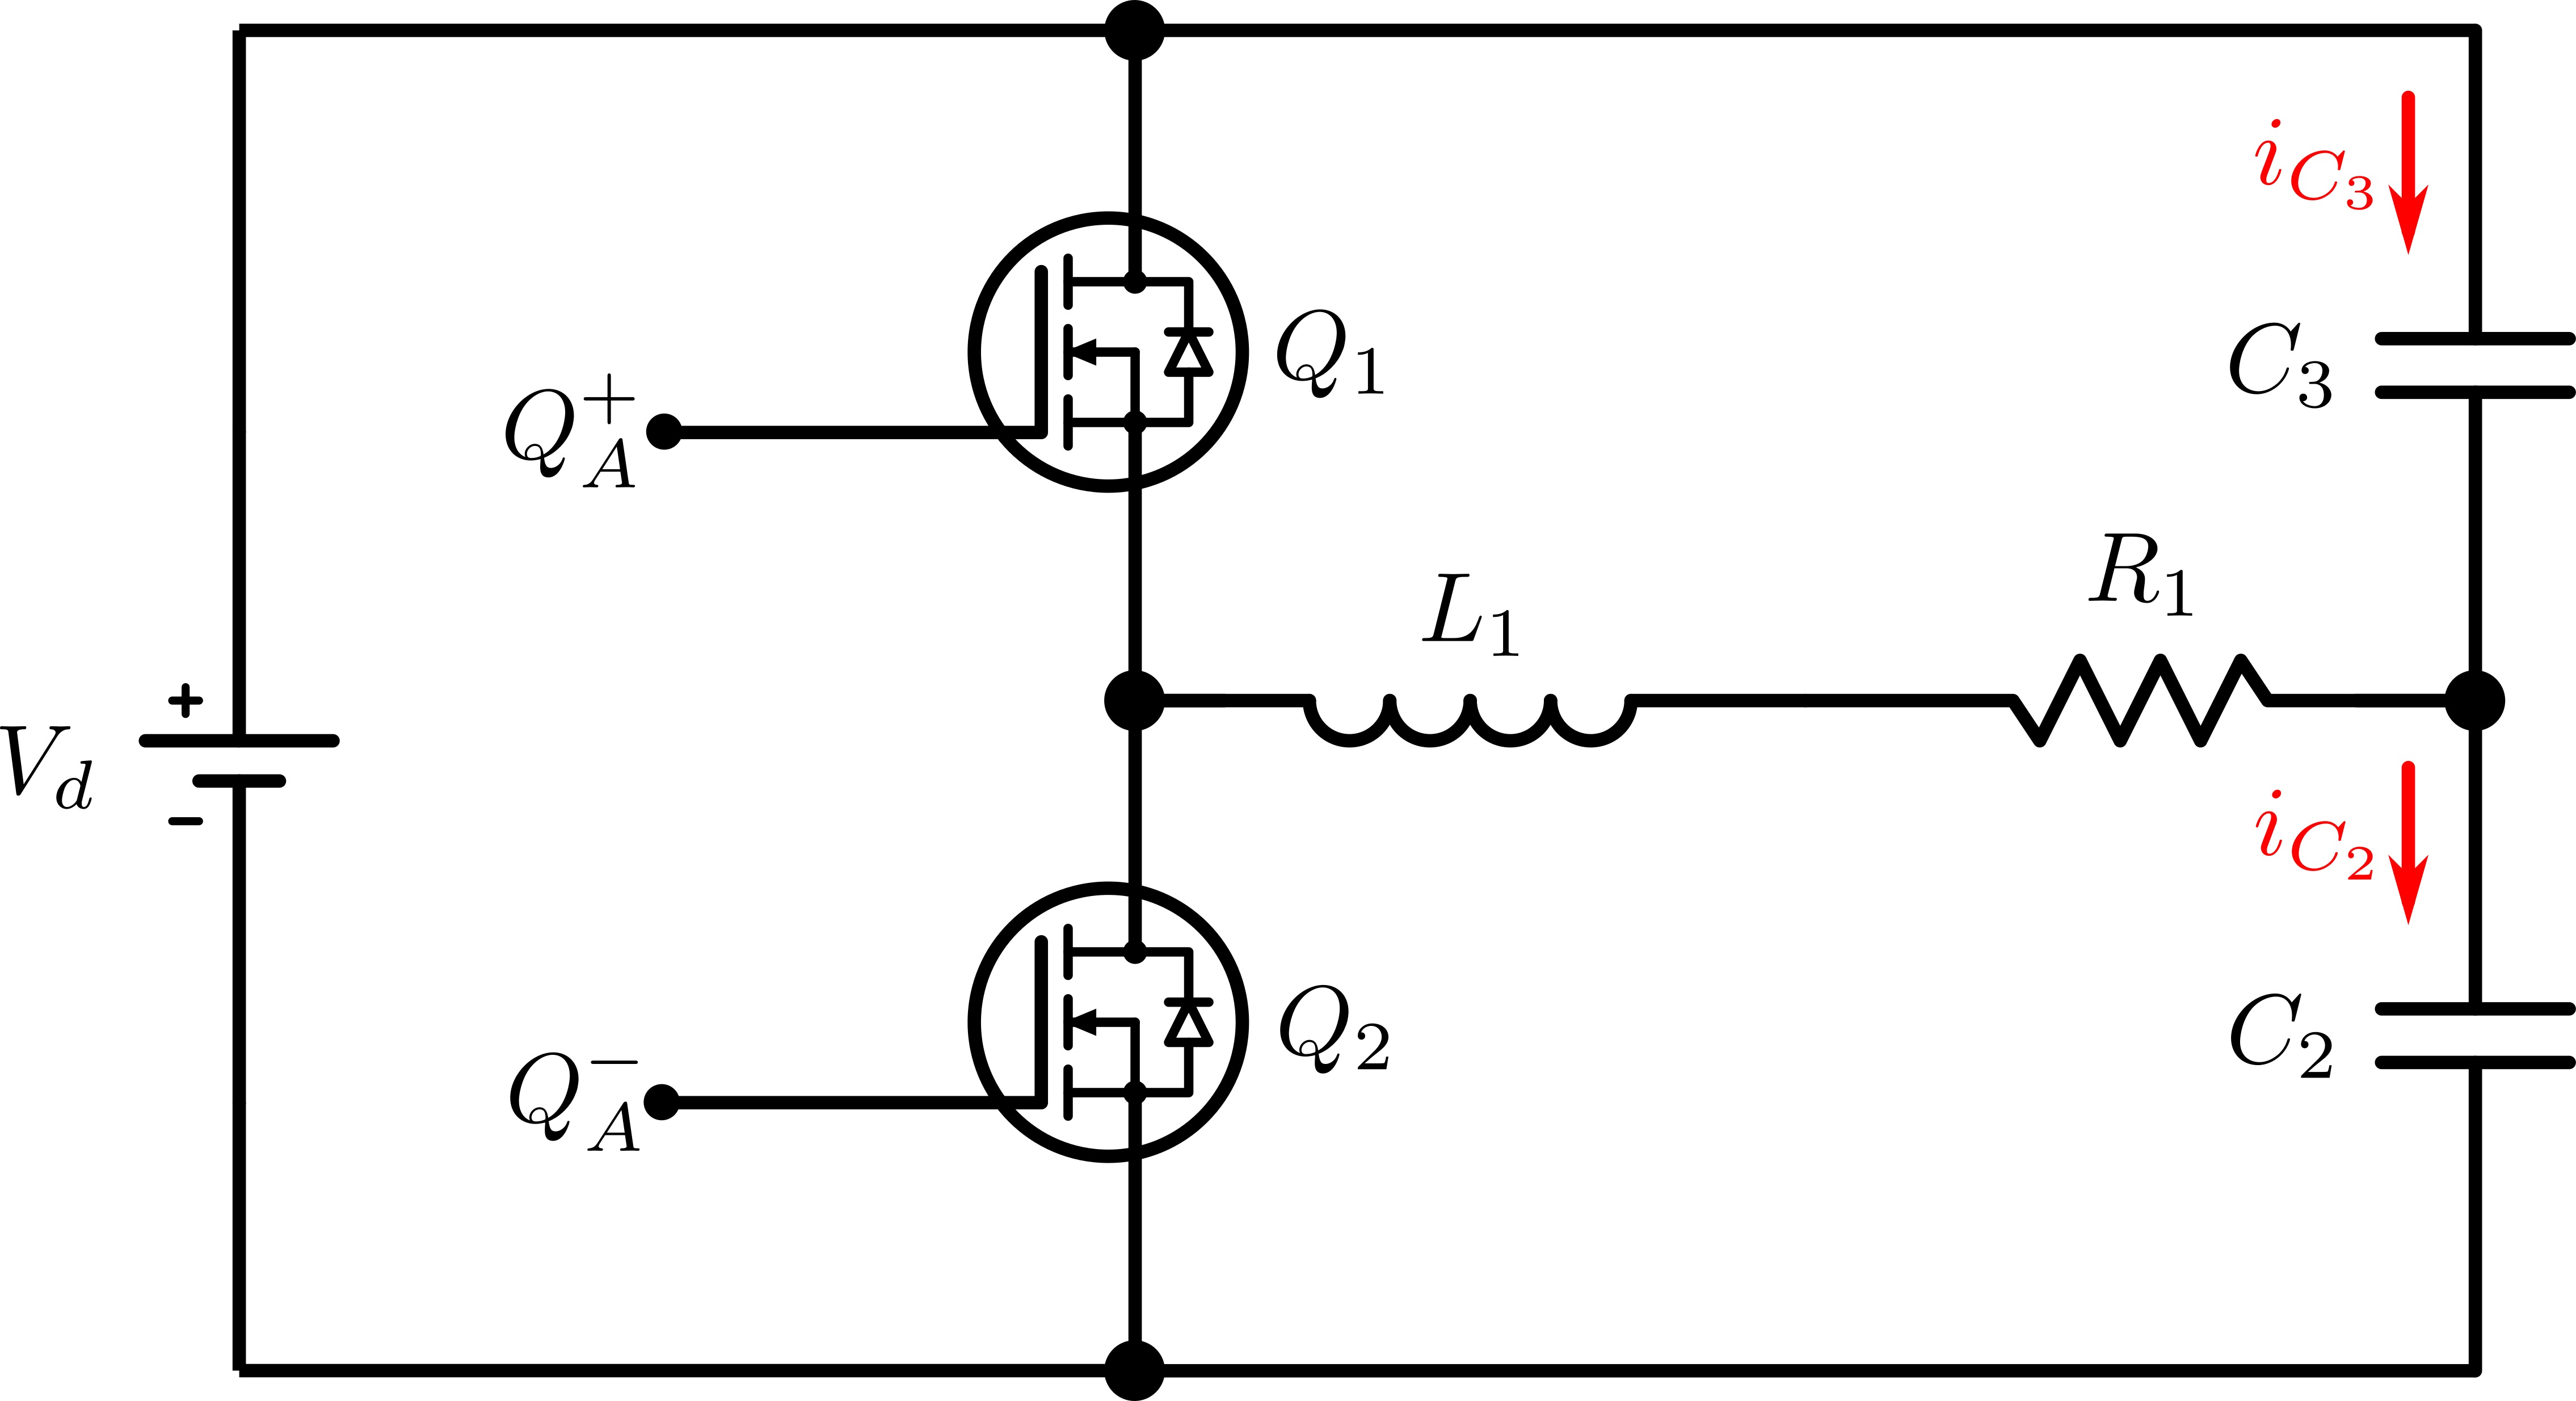
\includegraphics[width=0.8\linewidth]{Imagenes/parte1.png}
\caption{Inverter Monofásico}
\end{figure}

\begin{figure}[H]
\centering
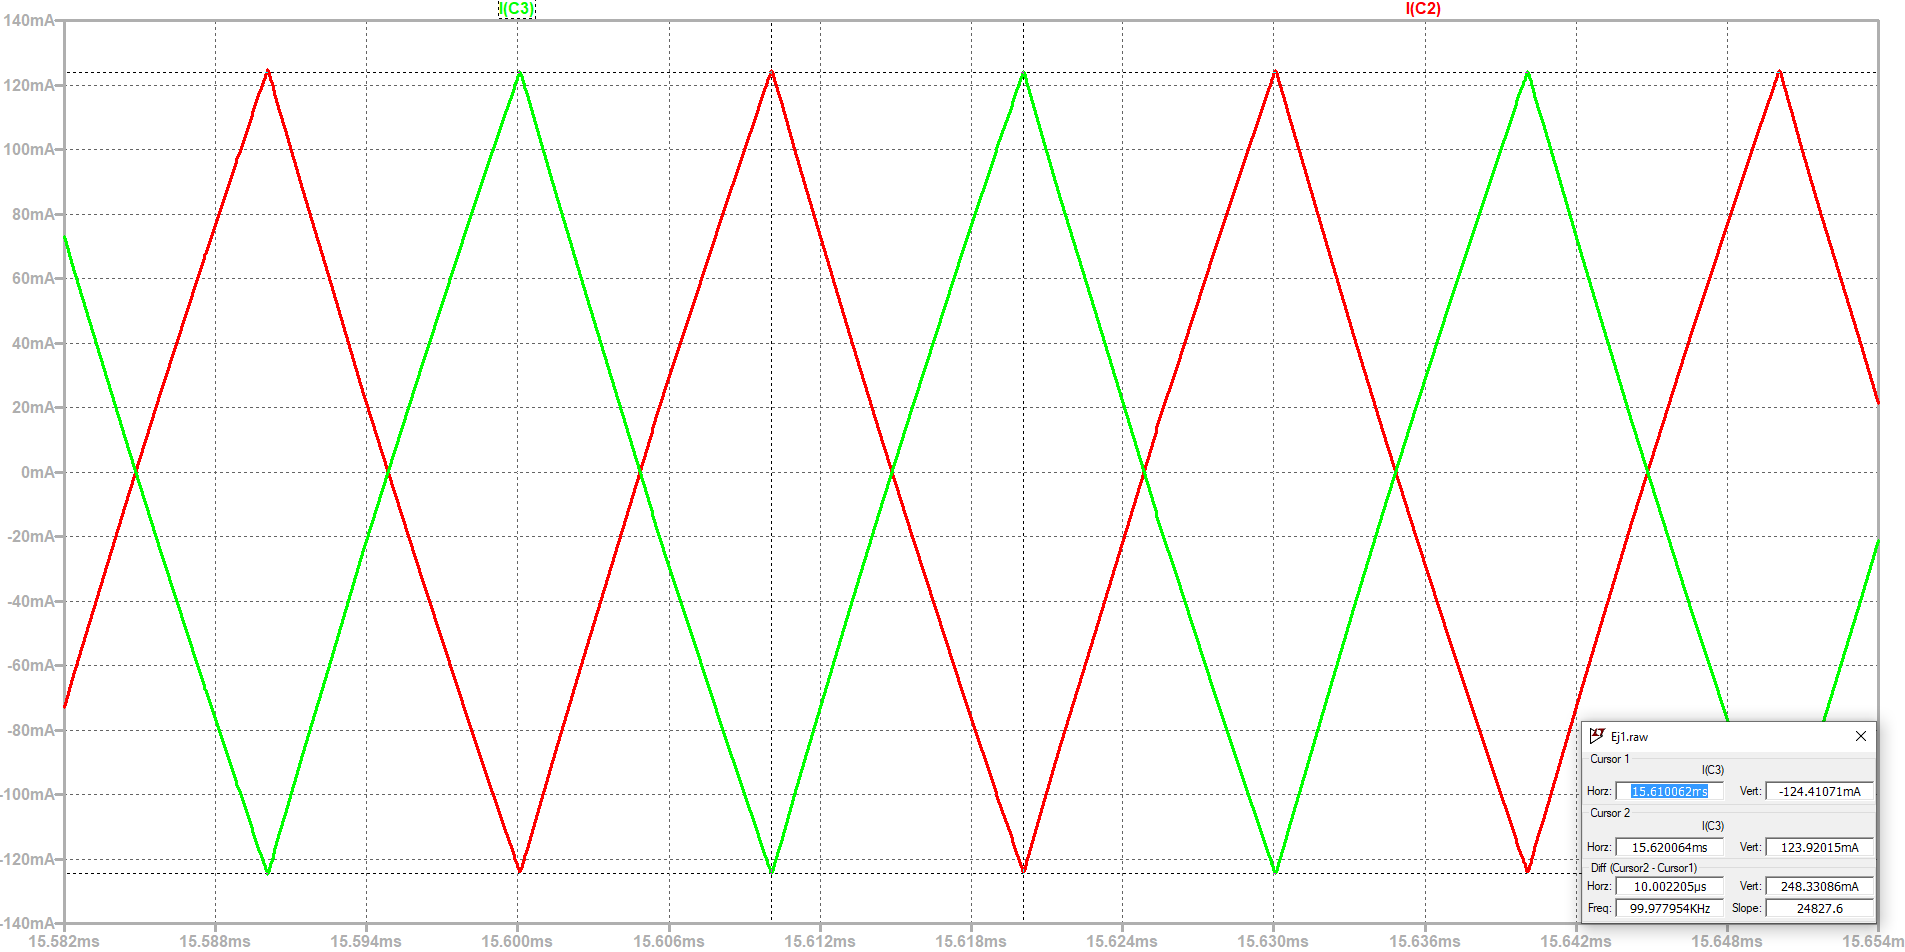
\includegraphics[width=0.9\linewidth]{Imagenes/corrientesC.png}
\caption{Circulación de corrientes por los capacitores}
\end{figure}

Cuando se enciende $Q_1$, la corriente circula a través de éste, por el conjunto $L_1 - R_1$ y por $C_2$ cargándolo positivamente, mientras que $C_3$ carga negativamente. Cuando se apaga $Q_1$ y se enciende $Q_2$, ocurre lo opuesto: ahora $C_2$ se carga negativamente y $C_3$ positivamente, manteniendo el valor medio de la corriente de ambos capactiores en 0, y la tensión prácticamente constante en ambos. La corriente en este caso circula a través de $C_3$, por el conjunto $L_1 - R_1$ y por $Q_2$.\par
A partir de lo anterior, a través de los diodos intrínsecos de los transistores no se tiene circulación de corriente estacionaria.

De la teoría, la expresión de la Serie de Fourier para una señal cuadrada con simetría impar que oscila entre -A y A es:

\[
x(t) \approx \sum_{k \in \mathbb Z (impar)}^{}X_k \cdot e^{ik\omega_0 t} = \frac{2A}{ik\pi} \cdot e^{ik2\pi \frac{t}{T}} 
\]

\todo[inline]{Ver que de parecido o igual en la fft}

\end{document}